\documentclass{article}

\usepackage[a4paper,margin=2cm]{geometry}
\usepackage{color, soul}
\usepackage{titlesec}
\usepackage{enumitem}
\usepackage{pdfpages}
\usepackage{multicol}

\title{SWEN30006 Assignment 2 - Report}
\date{\today}
\author{Workshop 09, Team 02\\Lucas Fern \& Cameron Maddern}

\begin{document}
\maketitle
This project required changes to be made to an existing Cribbage card game trainer system to add scoring and logging functionality. These additions were made with the use of a variety of design patterns in order to have minimum impact on the existing code, and therefore reduce coupling between existing classes and classes added for the new functionality.\\[2mm]
This report will discuss the changes which have been made, provide justification for the design patterns used, \hl{and argue in favour of these design patterns over the use of others where appropriate.} The additional classes will be covered first, then how these additional classes were integrated into the existing system.\\[2mm]
A class diagram of the updated design is included at the end of the report and will be relevant to visualise all changes to the system.

\section{Cribbage Observers}
In an effort to minimise coupling between added classes and maximise cohesion within them, a \verb|CribbageObserver| interface was implemented. This allowed classes to subscribe to various events of the Cribbage game, and respond with unique actions. This required the addition of a list of subscribers in the main \verb|Cribbage| class, as well as a method to register new subscribers.

\subsection{Cribbage Events}
Now that a publish-subscribe pattern is implemented it must be decided when events are broadcast to the subscribers. There are a variety of events in the game of Cribbage, and it was decided that all events which relate to the logging and scoring functionality will be broadcast to the subscribers. This allows - for example - the logging functionality for the \verb|deal| to be implemented by an observer responding to a \verb|Deal| event. The various subscribers to Cribbage Events are discussed further in section \ref{sec: crib subscribers}.\\[2mm]
The complete list of \verb|CribbageEvent|s implemented appears on the right side of the class diagram, and their functionality is briefly summarised below:
\begin{multicols}{2}
    \begin{itemize}
        \item \verb|SetSeed|\\[2mm]
        Subscribers are notified of this event when the game's seed is set from the \verb|cribbage.properties| file. The event contains the random seed which was chosen.
        \item \verb|InitPlayer|\\[2mm]
        This event is broadcast when the players of the game are initialised and assigned a number. This provides subscribers with information about the player type which has been initialised (\textit{eg.} \verb|cribbage.RandomPlayer|) and their number.
        \item \verb|Discard|\\[2mm]
        This event is created once for each player each game, when the player has selected which cards to discard. It provides observers with the players number, and a \verb|jcardgame.Hand| object containing the cards they selected for discarding.
        \item \verb|PlayStarter|\\[2mm]
        The \verb|PlayStarter| event is published once per game when the starter card is selected, and provides the starter card as a \verb|jcardgame.Card|.
        \item \verb|Play|\\[2mm]
        This event is raised on every turn of the game, when a player selects the card they wish to play. It contains the player's number, the card they played, and the total face value of the current board after adding this card.
        \item \verb|Show|\\[2mm]
        The \verb|Show| event occurs at the end of the game when play has ceased and players are showing card combinations from their hands to be scored. This event contains information about the player's number, the starter card, and the cards that they are showing to be scored.
    \end{itemize}
\end{multicols}
\begin{itemize}
    \item \verb|Score|\\[2mm]
    The \verb|Score| event is a special type of event raised by the Cribbage Scorer in response to other events, it occurs whenever a player's score is incremented, and contains data on the amount of points scored, their total score, and the type of score achieved. This will be discussed further in \ref{sec: crib scorer}
\end{itemize}


\subsection{Cribbage Subscribers}
\label{sec: crib subscribers}
\subsubsection{Cribbage Logger}
\subsubsection{Cribbage Scorer}
\label{sec: crib scorer}

% 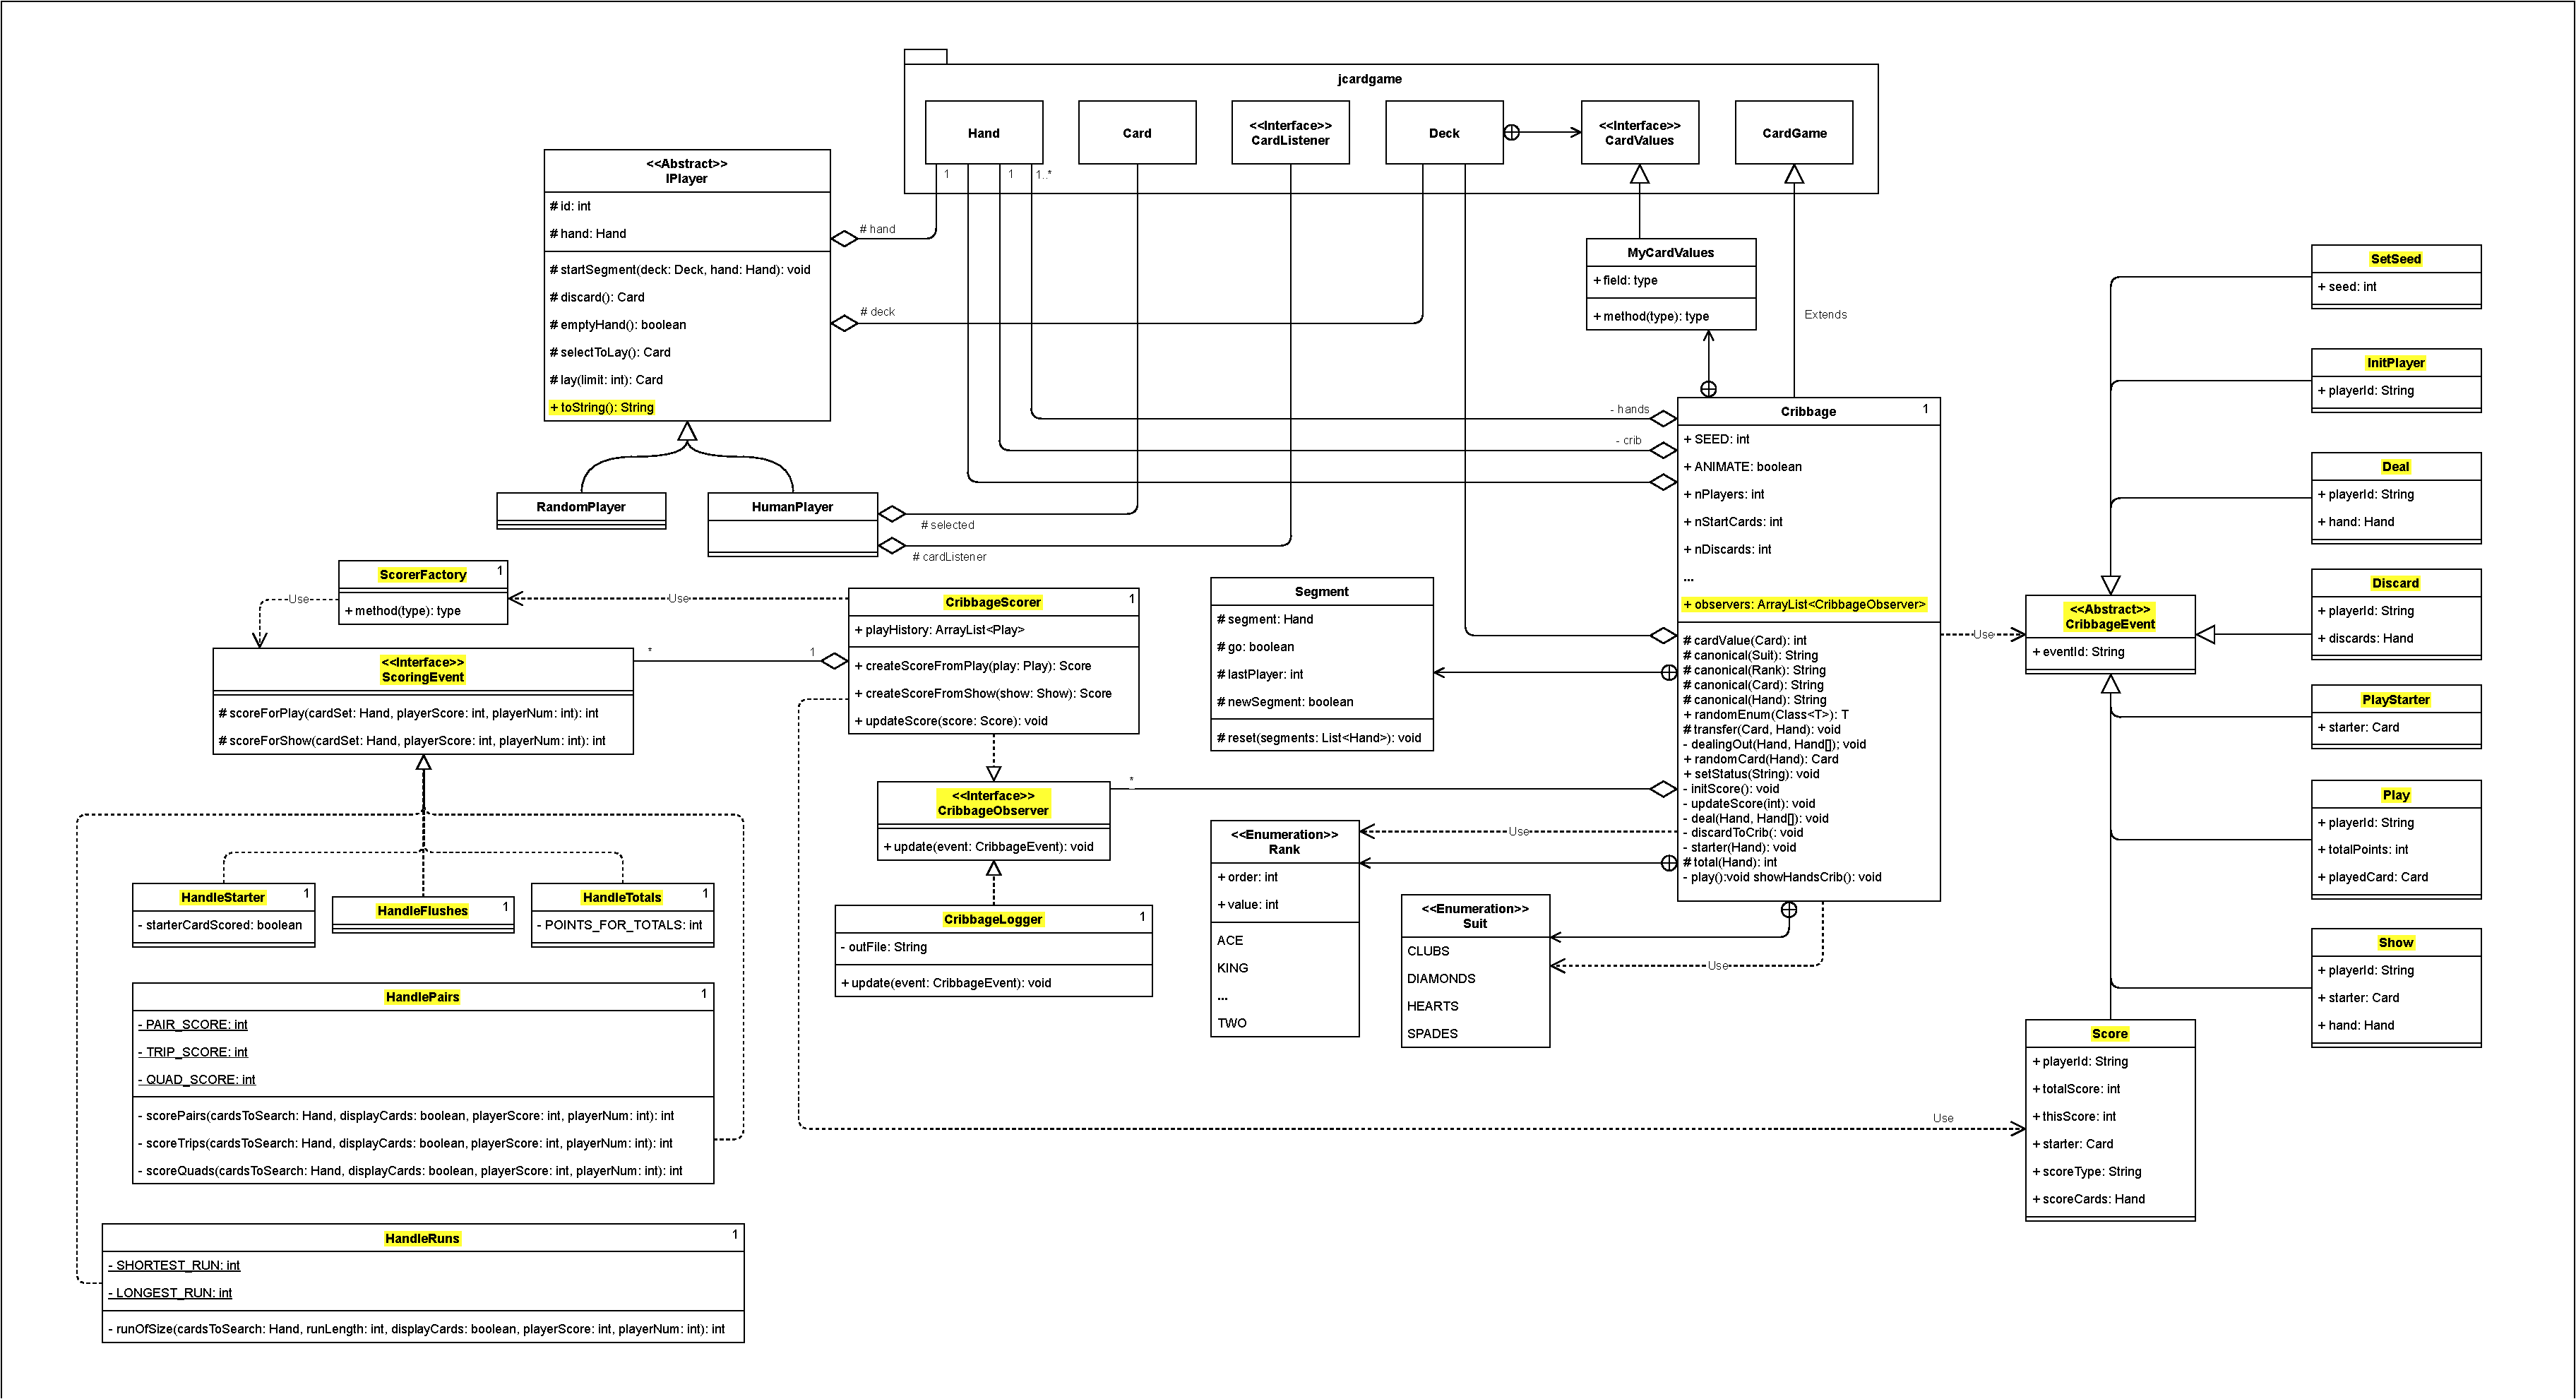
\includepdf[pages=-, fitpaper=true]{design-class-diag.pdf}
\end{document}